\chapter{Introduction}

\section{Motivation}
Revealing the structure of hierarchical organized data is a complex task where many approaches already exists (TODO cite). It is still an active research area as data scientists are facing ever greater challenges when analyzing large hierarchical datasets. One example is the Human Disease Network \cite{zhou_human_2014} which is a hierarchical network of disorders and disease genes with approximately 3000 nodes on two different hierarchy layers. Figure \ref{fig:Human_Disease_Network} shows us the representation of the data in a common two-dimensional layout, in this representation the classes of disorders are coded by color. 
Our own dataset with a similar structure can be seen in Figure \ref{fig:original2DdiseaseNet}, here the clusters of different diseases are grouped by boxes. Depiction of hierarchical network structure in 2D faces us with many challenges for example: 
\begin{itemize}
    \item \textbf{Limitation of visual features.} Figure \ref{fig:Human_Disease_Network} already uses the color to encode the group membership thus we can not use a color scale to visualize additional attributes like mortality rate.
    \item \textbf{Lack of space.} A common problem in network visualization is the hairball effect, with only two dimensions the reduced space quickly leads to overlapping of nodes and links. In Figure \ref{fig:Human_Disease_Network} we can see this effect on the green nodes. The graph in Figure \ref{fig:original2DdiseaseNet} solves this problem by hiding links between child nodes from different boxes which is also not optimal.
    \item \textbf{Restriction of spatial encoded data.} With only two available axes and therefore only two spatial encoded data attributes task like cluster detection and conformation are harder.
\end{itemize} 

\begin{figure}[h]
    \centering
    \begin{subfigure}[b]{0.4\columnwidth}
        \centering
        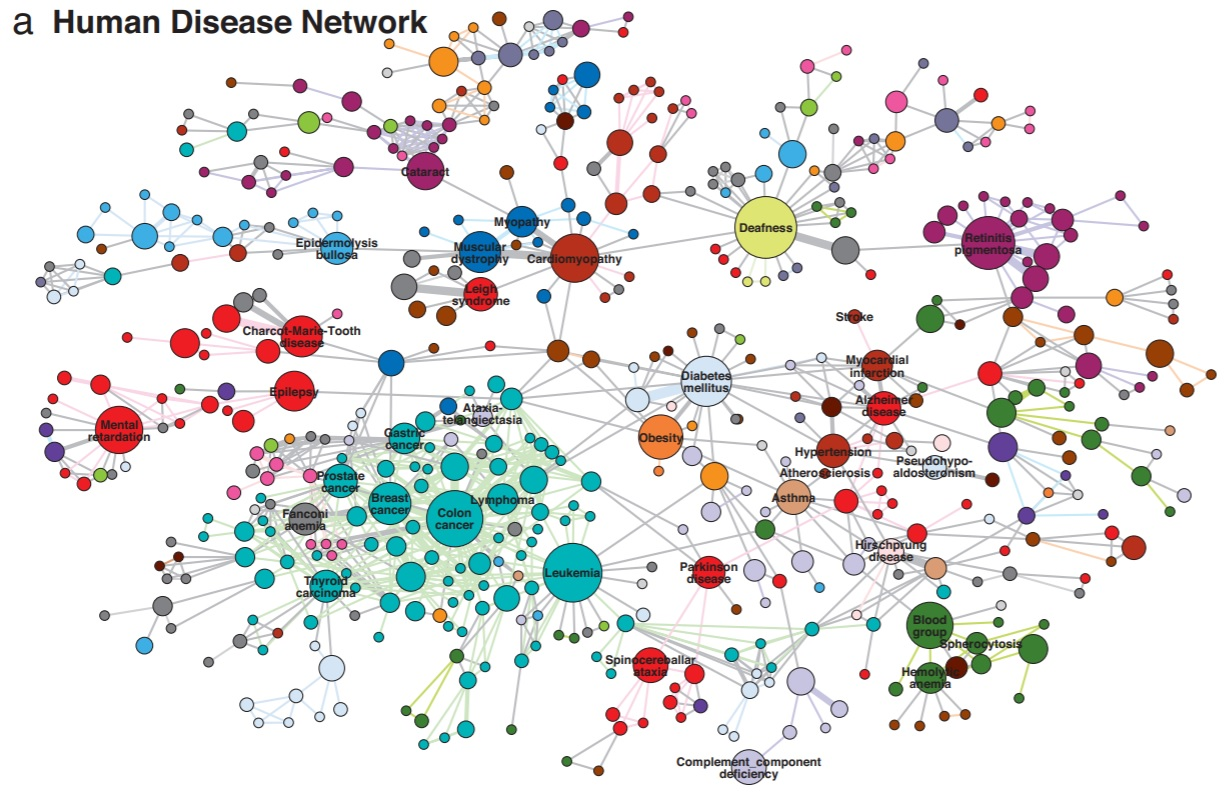
\includegraphics[width=\textwidth, trim={0 0 9cm 0},clip]{graphics/Human_Disease_Network.jpg}
        \subcaption{Human Disease Network \cite{zhou_human_2014}}
        \label{fig:Human_Disease_Network}
    \end{subfigure}
    \begin{subfigure}[b]{0.5\columnwidth}
      \centering
      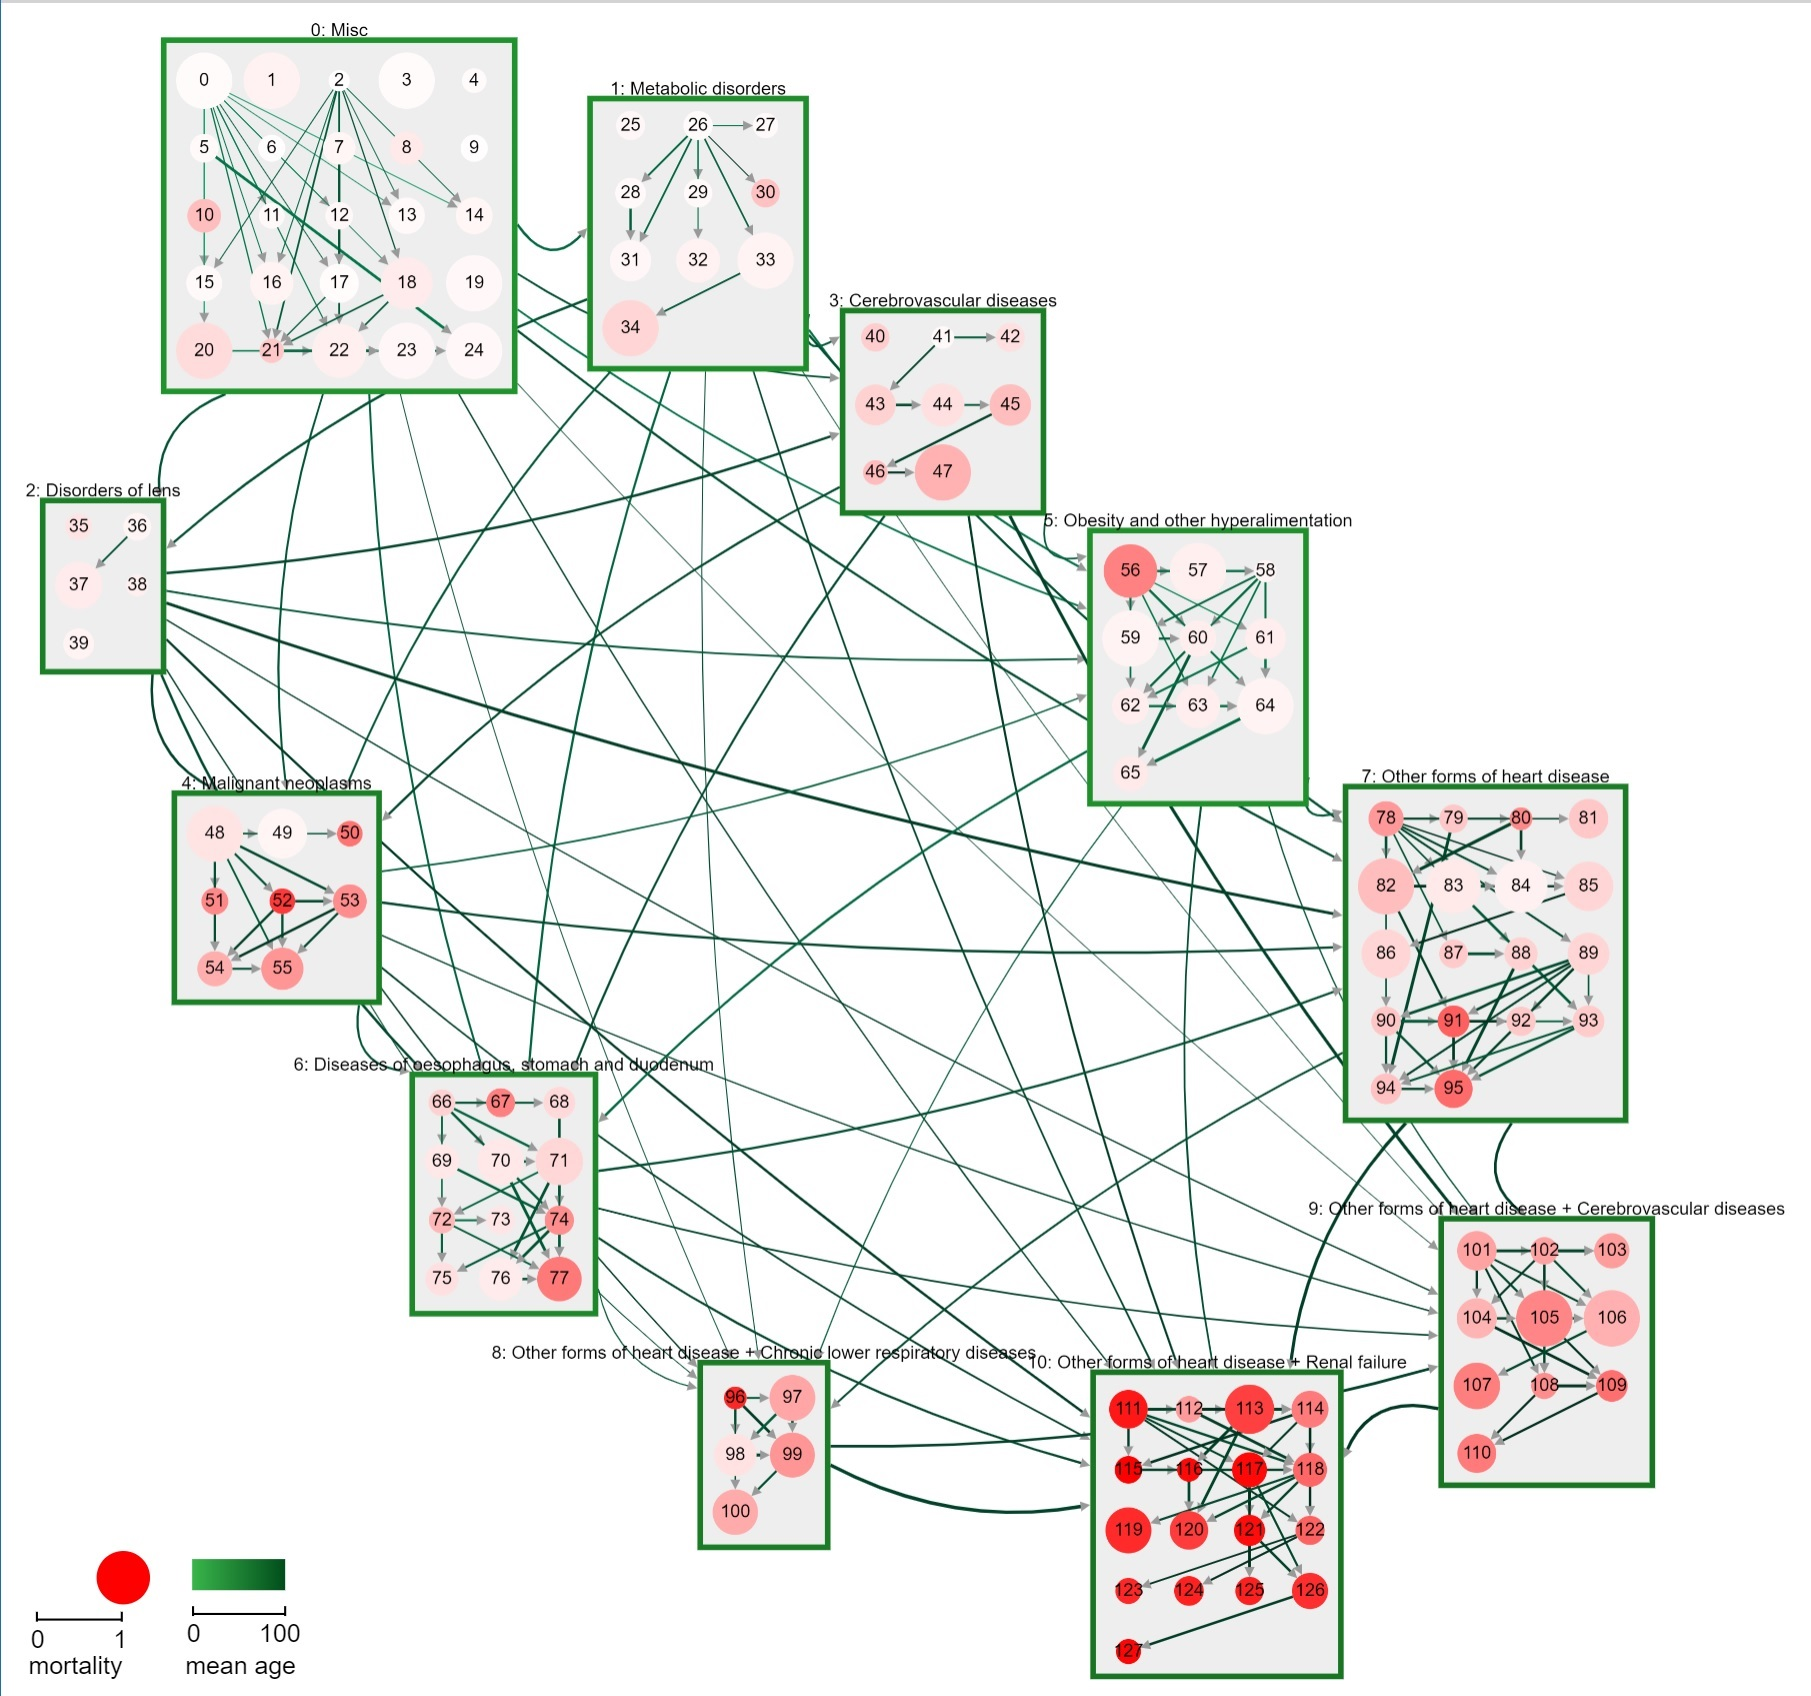
\includegraphics[width=\textwidth]{graphics/original2DdiseaseNet.jpg}
      \subcaption{Our own disease network dataset}
      \label{fig:original2DdiseaseNet}
    \end{subfigure}
    \caption[Optional caption for the figure list (often used to abbreviate long captions)]{Example visualizations of hierarchical network datasets in two dimensions. Both consists of two hierarchical layers.} % Remove the [...] argument if the original caption should be used in the figure list.
    \label{fig:intro} 
  \end{figure}

3D information visualization allows us to expand the user experience of traditional 2D graphs. As Brath describes in his paper \cite{brath_3d_2014} there are many advantages and opportunities when using three-dimensional visualizations.
The additional axes allow us to encode an additional attribute by its position, this can be seen in the “3D space time cube” \cite{brath_3d_2014} here the temporal information is encoded on the Z axis another common usage is a 3D scatter plot. By using these additional spatial information the mental model gets improved. Furthermore, this results in a better understanding of the data by the user.
In the context of visual features we get a lot more of opportunities, one of the biggest is probably the ability to use surfaces and effects like shading. 
The perspective of the visualization can be reconsidered. Usually the user looks from the outside with a
bird's eye view at the visualization. In 3D however the viewer can be placed right inside our graph, this enables us to utilize new navigation and interaction possibilities. 

Still, all these opportunities also involve new challenges: navigation inside the visualization, occlusion of elements in an 3D perspective view, selection for displaying details and the lack of a reference point in three-dimensional space. Brath \cite{brath_3d_2014} already stated that immersive interfaces could help to overcome this issues.
 We believe that with the recent developments in virtual reality hardware and frameworks these challenges can now be solved even better. 
 We can see the benefits of VR based visualizations in various publications. Bowman et al. \cite{bowman_virtual_2007} examined the impact of VR techniques like stereoscopic images, interaction with the virtual world and head movement can have on users. 
 Recently Kraus et al. \cite{kraus_impact_2020} did a study on the effect of immersion for detecting clusters in a scatter plot. Their results show that VR based visualization systems have real world advantages in terms of time needed to get an overview of the data compared to traditional 2D- and 3D information visualization. In terms of navigation and interaction Yang et al. \cite{yang_embodied_2020} explored the possibility of zooming and rotation of an entire graph and Drogemuller \cite{drogemuller_examining_2020} compared different navigation concepts.
 
 \section{Methodology}

Our concept is to take existing already good examined visualizations and extend them by one dimension, furthermore solving the subsequent challenges of 3D info visualization by using VR based technology and applying refined techniques for navigation and interaction. 
In addition, our visualization concept should not only work with two hierarchical datasets as used in our demo dataset from Figure \ref{fig:original2DdiseaseNet} but rather it should be able to display $n$ hierarchical layers.

We got inspired by a circular form of a tree map plot for hierarchical structures see Figure \ref{fig:hierarchicalCirclePlot}. However, the nodes $\{A,B,C,\dots\}$ are only simple attributes but in our data structure each node can either be a simple leaf node or a network itself. So we need a way to visualize connections between different networks, a way to do this is a multilayer network visualization see Figure \ref{fig:2dmultilayerVis}. Here each flat layer represents a different network but a hierarchical relationship is not always given for these visualizations.  

\begin{figure}[h]
    \centering
    \begin{subfigure}[b]{0.40\columnwidth}
        \centering
        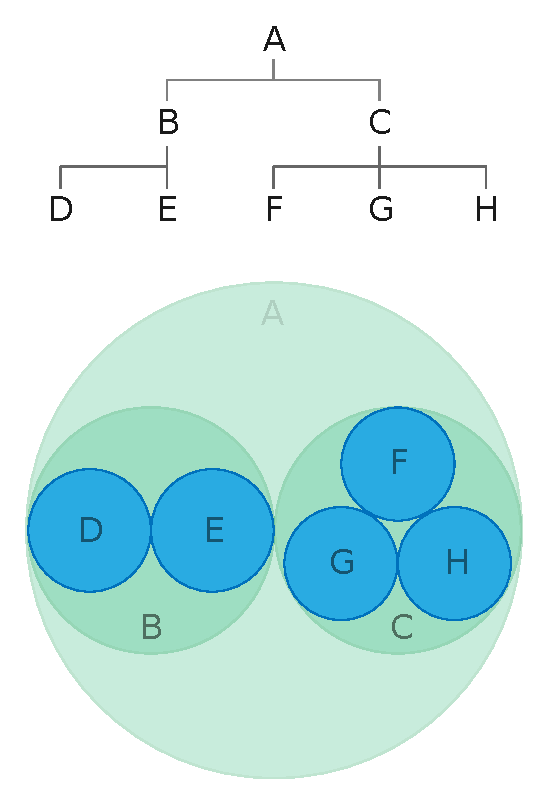
\includegraphics[width=\textwidth, trim={0 0 0 4.3cm},clip]{graphics/circle_packing.pdf}
        \subcaption{Hierarchical circle packing plot \cite{ribecca_circle_nodate}}
        \label{fig:hierarchicalCirclePlot}
    \end{subfigure}
    \begin{subfigure}[b]{0.50\columnwidth}
      \centering
      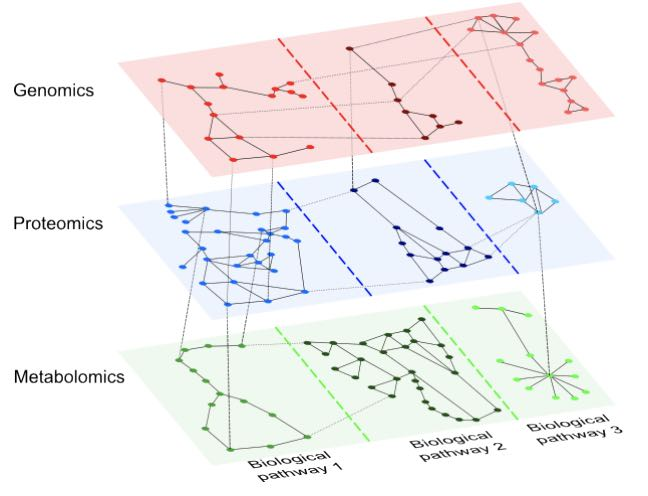
\includegraphics[width=\textwidth]{graphics/2dmultilayerVis.jpg}
      \subcaption{multilayer network visualization \cite{ghoniem_state_2019}}
      \label{fig:2dmultilayerVis}
    \end{subfigure}
    \caption[Optional caption for the figure list (often used to abbreviate long captions)]{Reference visualizations that we used as a starting point. (a) shows a possible visualization for hierarchical structures, (b) shows a visualization for networks with multiple layers} % Remove the [...] argument if the original caption should be used in the figure list.
    \label{fig:referenceVisualizations} 
  \end{figure}

We combined the concepts of both plots, see Figure \ref{fig:conceptSketch}: 
\begin{itemize}
    \item Instead of rendering each layer from the multilayer plot as a flat surface we use a three-dimensional structure instead, so we can make use of the whole volume for our network layout. More specifically we use a sphere for each node.
    \item For the hierarchical relationship we use the concept of nesting as seen in the circle packing plot. However, we use 3D spheres instead of 2D circles. 
    \item Links between nodes are possible in one network but also to other networks of the same hierarchical layer.   
\end{itemize}

\begin{figure}[h]
    \centering
    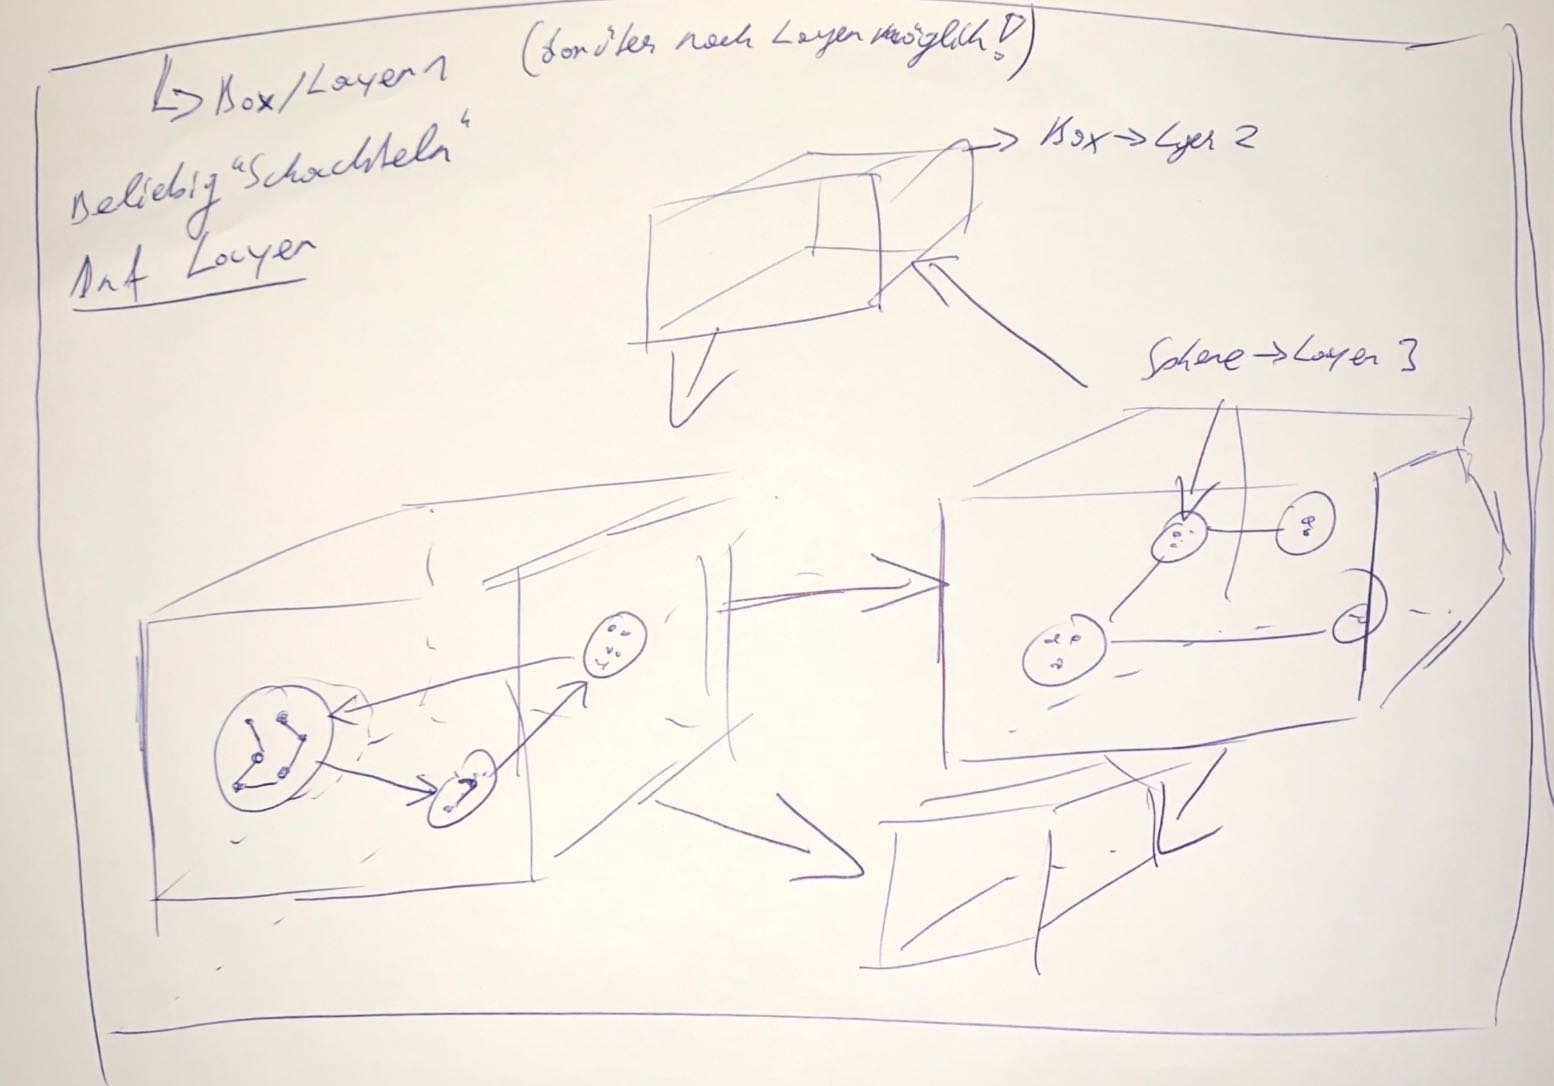
\includegraphics[width=1\textwidth]{chapters/graphics/concept1.jpg}
    \caption{TODO screenshot from the visualization with the dataset from \ref{fig:original2DdiseaseNet}} % Remove the [...] argument if the original caption should be used in the figure list.
    \label{fig:conceptSketch} 
\end{figure}

For navigation, we allow the user to dive right into our graph. Therefore, we provide two kinds of navigation methods: One for bridging larger distances like flying to a specific node selected by the user or flying to the hierarchical parent node. Additional, a free flying navigation that allows the user to fine tune their position. To prevent occlusion we render the nested nodes transparent and use a collision constraint to prevent collisions in the same hierarchical layer. Filtering and brushing methods are used to prevent overlapping of links these are triggered automated by the users position and also can be activated manually by interaction. Selection of nodes is possible with a “laser pointer” attached to the user's controller. Lastly we also allow the user to change the scale of the entire scene, this is useful as we can not know the users physically available space to move in the virtual environment and their spatial impression preferences. 


\section{Aim of the Work}
%From proposal: \\
%The	 goal	 is	 to	 visualize	 a	 hierarchical	 network	 with	 n	 Layers.	 Each	 Node	 in	 a	 graph	 can	
%represent	a	graph	itself.	There	are	multiple	examples	where	this	has	been	visualised	in	2D,	
%however	we	believe	that	with	an	additional	dimension	and	when	3D	graphs	are	analysed	in	
%VR	we	can	get	even	more	insight	and	a	better	overview	of	the	data.	

Ideas:
\begin{itemize}
    \item provide a prototype application
    \item benefits of webbased implementation 
    \item experiment with different concepts/approaches
    \item experiment with different interactions
    \item ...
\end{itemize}

\begin{quotation}
    However, there is considerable value in research that
    solves a well-motivated problem using a combination
    of preexisting solutions 
\end{quotation}
Sadana\\
Redefining a Contribution for Immersive Visualization Research\\